\documentclass{swfcthesis}

\addbibresource{bb.bib}    % 参照教程自己去写一个.bib文件

\begin{document}

\Title{操作系统探索}
\Author{尹志成}
\Advisor{王晓林}
\AdvisorTitle{讲师}
\AdvisorInfo{王晓林,男,49 岁,硕士,讲师,毕业于英国格林尼治大学,分布式计算系统专业。
  现任西南林业大学计信学院教师。执教 Linux、操作系统、网络技术等方面的课程,有丰富的 Linux 教学和系统管理经验。}
\Month{六}
\Year{二〇一八}
\Subject{计算机科学与技术专业}    %专业名称(比如 计算机科学与技术专业)
\Abstract{操作系统最初的诞生是为了搭配进行简单繁重的数字运算机,但随着时代的演进,
  计算机不仅作为处理各种运算的机器,其附加价值也越来越被人们看重,跟随着计算机的发展,
  操作系统的使命也在一代代的改变,(约两百字)}
\Keywords{操作系统}
\Acknowledgments{感谢,}
\enTitle{Operating system exploration}
\enAuthor{Zach Yin}
\enAbstract{英文摘要}
\enKeywords{Operate System}

%%% 下面六行不要动!
\makepreliminarypages% 封面
\frontmatter          
\tableofcontents     % 目录
\listoffigures       % 插图目录
\listoftables        % 表格目录
\mainmatter

% 引言
\chapter{绪论}
在数字时代,操作系统的重要性不言而喻,它作为计算机软硬件之间的桥梁,存在于日常生活的每一个角落,
而研究一个只有庞大的公司聚集成百上千的高级工程师才能完成的操作系统对于学生而言是一个几乎不可能完成的挑战,
但是克服难关是锻炼技术的必经之路\cite{30_os},所以研究并完成一个基本满足日常功能需求的操作系统作为此次的目标,
并以此为跳板对操作系统进行更深一步的探究。

% 思路
\chapter{思路}

此次的思路由四部分组成:
\begin{enumerate}
    \item 操作系统探究
    \item 空白操作系统的启动
    \item 编写操作系统内核
    \item 实现对外兼容及安全防护
    \end{enumerate}

\section{操作系统探究}
从历史上计算机操作系统的发展联系到人们的日常生活,寻求符合操作系统发展且适应用户使用的特征要素。

\section{空白操作系统的启动}
利用汇编语言及操作系统相关知识探究操作系统如何从电气设备到软件代码的衔接。

\section{编写操作系统内核}
从内存管理,输入输出,多进程,分时四个模块完成操作系统的内核设计及实现。

\section{实现对外接口及安全防护}
从接口设计及安全防护的角度完善操作系统。

% 原理
\chapter{操作系统探索}

\section{操作系统的诞生}

\subsection{第一代:真空管}

操作系统最初出现的场景是一个工程师小组设计、建造一台机器,之后使用机器语言编写程序并通过将上千根电缆接到插线板上连接成电路,
控制机器的基本功能,进而操作机器运算诸如制作正弦、余弦、对数表或计算炮弹弹道的简单数学运算。

这里的人工拔插电缆就充当着操作系统的角色——根据程序直接操作硬件使其运算得出结果。

% -------------

\subsection{第二代:晶体管}

在晶体管发明后,计算机可靠程度大大增加,计算机开始被一些公司、政府部门或大学使用。

改进后出现了操作系统的载体,卡片和较后期磁带打孔纸带。

由于打孔纸带是分次读入,一次只能读入一个的作业,出现了批处理系统如图~\ref{fig:btss}: 

\begin{figure}[h]
  \centering
  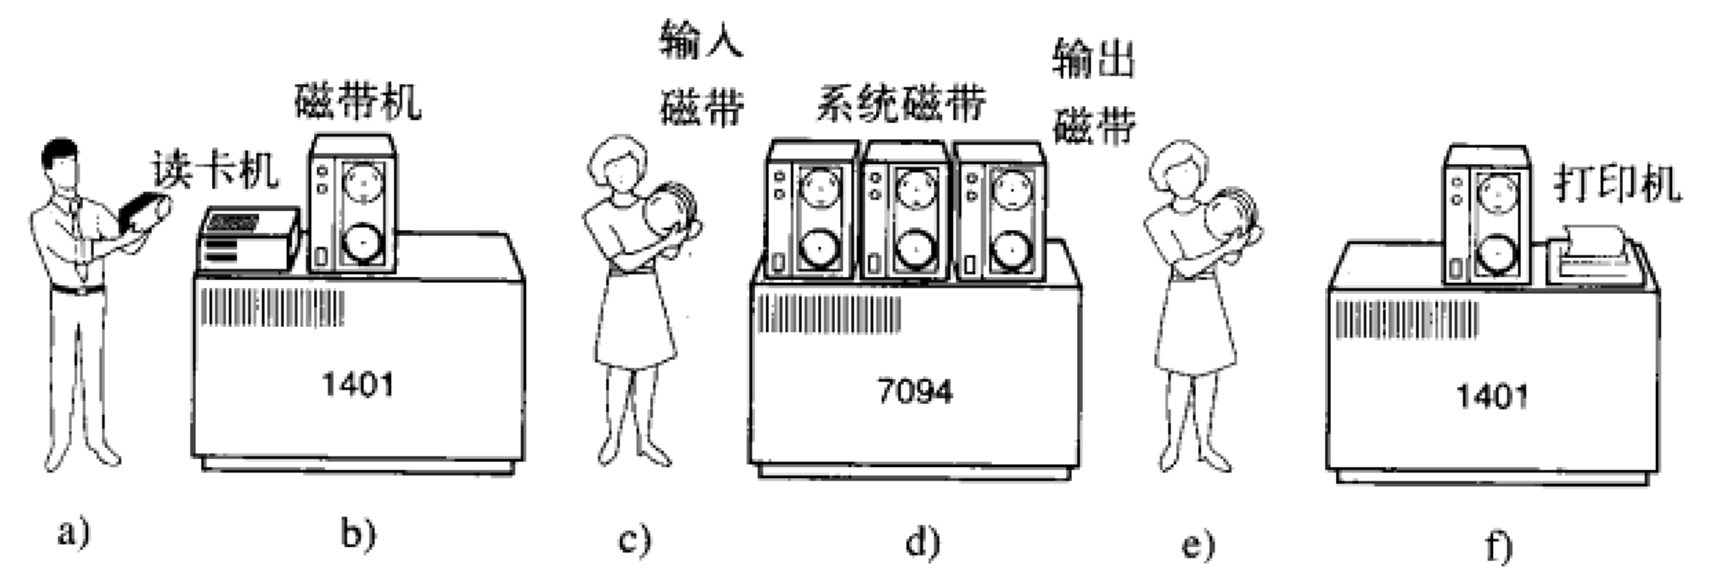
\includegraphics[width=.8\textwidth]{fig/btss.png}
  \caption{批处理系统}
  \label{fig:btss}
\end{figure}

\begin{description}
\item[a.]程序员将打孔纸带拿到1401机\footnote{IBM 1401:数据处理计算机\cite{1401dps}}
\item[b.]1401机将批处理作业读到磁带上
\item[c.]操作员将输入磁带送至7094机\footnote{IBM 7094:专为大型科学计算而设计,具有出色的性价比和扩展的计算能力\cite{7094dps}}
\item[d.]7094机进行计算
\item[e.]操作员将输出磁带送到1401机
\item[f.]1401机打印输出
\end{description}

在这里,操作系统的工作已经由完全的人工转换到一部分人工操作交由机器完成,工作效率较之前大大提高,
并且,由于加入了磁带,计算机完成的工作也将及时得到保存。

操作系统的工作已经开始有一定的流程化了。

% -------------

\subsection{第三代:集成电路}

采用集成电路的第三代计算机较分立晶体管的第二代计算机在性能/价格比上有了很大的提高,

第三代操作系统加入了多道程序设计和分时系统,可以适应多道程序同时运行的任务。
\begin{enumerate}
  \item 多道程序设计主要目的是解决CPU因等待磁带或其他I/O操作而暂停工作,多道程序设计可以使CPU在程序a的I/O操作时运行程序b\cite{tanenbaum2009modern}。
  \item 分时系统解决的主要问题是多用户使用分离的终端,却操作同一台计算机。
\end{enumerate}

% -------------

\subsection{第四代:个人计算机}

大规模集成电路进一步减小了计算机的大小,进一步为计算机进入大众视野做好了铺垫。

现在使用的台式机和笔记本就是属于第四代计算机发展的较高版本。

第四代计算机和之前的计算机比较而言在于同一台终端的使用人数,
第四代之前的计算机主要用于科研和大规模计算,所有硬件都是为这些作业而工作,操作系统也只用为这些作业安排调度,
而每个人都能拥有自己的计算机,那么计算机就需要有更多个性化的东西,这对操作系统提出了更多的要求:

\begin{enumerate}
  \item 更多的进程
  \item 更大的存储空间(文件管理)
  \item 更多设备接入(如鼠标)
  \item 网络要求的实现
  \item 对外防护的要求
  \item 对外提供接口(图形化显示)
\end{enumerate}

% -------------

\subsection{第五代:移动计算机}

第五代计算机是便携式计算机,也就是智能手机或者智能平板设备,较之第四代计算机最大的不同在于易于携带,
但是缺点也很显著,受到设备体积和电池的限制,性能受到很大的影响。

第五代计算机对操作系统有了新的要求:
\begin{enumerate}
  \item 从待机状态极快的响应
  \item 电量控制(即低成本完成作业)
\end{enumerate}

% ----------

\subsection{总结}

纵观操作系统的发展史,发展的中心问题是“如何更低成本完成更多的任务”,
而发展的关键节点是多道程序设计以及分时系统。

展望计算机的发展史,大胆的推测下一代计算机可能就是"computer everywhwere",
而那时操作系统也会有新的发展。

\section{操作系统的规范化}

\subsection{Unix及类Unix}
Unix 及类 Unix 将用户空间与系统空间划分开,以此规定内核的边界,将存在于系统空间的代码与数据的集合称为内核。
由此也存在了不同的 CPU 运行模式:系统态和用户态。
\begin{enumerate}
  \item 系统调用接口
  \item 进程管理
  \item 内存管理
  \item 虚拟文件系统
  \item 网络堆栈
  \item 设备驱动程序
\end{enumerate}

\subsection{Windows}

Microsoft Windows 与 Unix 最大的不同是,它将较低层的离硬件最近的一部分叫做“内核”,
因此,Windows也将图形界面和视窗机制的实现也放在了内核中。

大体来说,Windows内核层次如下:
\begin{enumerate}
  \item 系统调用接口
  \item 中断/异常入口
  \item Executive (管理层)、对象管理、内存管理、进程管理、安全管理、I/O管理等~\cite{毛德操2005windows}
  \item 核心层、设备驱动底层
  \item HAL(硬件抽象层)
\end{enumerate}

\subsection{小结}
从市场中用户数量较多的两大操作系统平台看,操作系统已经趋于规范化,功能方面也趋于成熟,
两大操作系统的功能都非常完备,但功能多了的坏处就是bug出现的概率也随之变高,
所以windows的蓝屏和linux的系统抖动等操作系统问题都对用户造成了极大的困扰。

想要解决这些问题较好的办法就是精简功能,从降低代码数量开始降低系统bug的出现概率,
精简功能则要很好的处理好必要功能和非必要功能的筛选分类。

% 启动
\section{启动空白操作系统}

\subsection{操作系统启动流程}

按下电源键后计算机开始启动,启动过程分为3个阶段~\cite{阮一峰2014如何变得有思想}:
\begin{center}BIOS -> MBR -> 操作系统\end{center}

\begin{enumerate}
\item 在BIOS完成POST(硬件自检,Power-On Self Test)
  并根据启动顺序(Boot Sequence)来选择启动设备。本系统是从U盘启动。
\item 计算机读取该设备的MBR(Master boot record,位于第一个扇区,即最前面的512个字节,如图~\ref{fig:mbr}所示),
  并运行其中的启动程序IPL(Initial Program Loader),将ZOS加载入内存。
  本部分的实现代码,参见附录程序~\ref{sec:ipl09}。
\item 控制权转交给操作系统后,Kernel开始运行,操作系统启动完成。
\end{enumerate}

\subsection{制作MBR}

MBR的主要部分是Bootstrap code area,即前446个字节。MBR结构如图~\ref{fig:mbr}所示。
负责指出操作系统的位置,主分区第一个扇区的物理位置(柱面、磁头、扇区号等等)
,实现如附录程序\ref{sec:fat12}所示。

\begin{figure}[H]
  \centering
  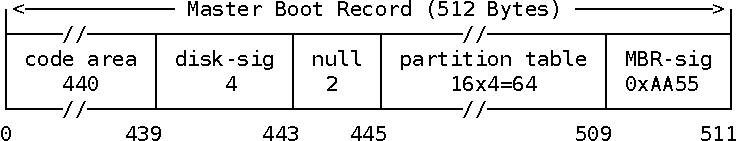
\includegraphics[width=1\textwidth]{../Fig/mbr.pdf}
  \caption{MBR}
  \label{fig:mbr}
\end{figure}

一个扇区大小为512字节,MBR位于C0-H0-S1(柱面0,磁头0,扇区1),\cite{刘伟2010数据恢复技术深度揭秘}
从下一个扇区(扇区2,C0-H0-S2)开始加载操作系统。找到扇区2的代码参见程序~\ref{lst:chs}。

\begin{listing}[H]
  \begin{codeblock}[.5]
  \inputminted[tabsize=2, firstline=43, lastline=45,
  linenos=true]{nasm}{../ZOS/src/kernel/ipl09.nas}
  \end{codeblock}
  \caption{初始化读取柱面、磁头和扇区的起点}
  \label{lst:chs}
\end{listing}

完成定位后开始将磁盘数据读入内存,策略是
\begin{enumerate}
\item 磁头0,柱面0,读取1-18扇区 (C0-H0-S2)-(C0,H0,S18)
\item 磁头1,柱面0,读取1-18扇区 (C0-H1-S1)-(C0-H1-S18)
\item 磁头0,柱面1,读取1-18扇区 (C1-H0-S1)-(C1-H0-S18)
\item ...
\item 磁头1,柱面78,读取1-18扇区 (C78-H1-S1)-(C78-H1-S18)
\item 磁头0,柱面79,读取1-18扇区 (C79-H0-S1)-(C79-H0-S18)
\item 磁头1,柱面79,读取1-18扇区 (C79-H1-S1)-(C79-H1-S18)
\end{enumerate}

按以上策略将磁盘内容读入内存,核心代码参见附录程序~\ref{sec:readfrag}。

readfast 位于代码第76行,JMP readfast 在此代表循环执行。
当循环执行完毕,表示磁盘内容已经全部加载到内存中,
MBR过程成功,开始启动操作系统。

\subsection{制作空白操作系统}

为测试操作系统是否成功被MBR启动,设计将操作系统设置为启动后待机。
本部分的实现代码,参见程序~\ref{lst:blankos}。按下电源键,经过启动步骤系统循环执行
HLT\footnote{HLT: 让CPU停止动作并进入待机状态\cite{30_osKawaiHidemi200630}}
使得操作系统计算机始终处于待机状态,启动成功。

\begin{listing}[H]
  \begin{codeblock}[.5]
    \begin{nasmcode}
      fin:
      HLT
      JMP fin
    \end{nasmcode}
  \end{codeblock}
  \caption{空白操作系统}
  \label{lst:blankos}
\end{listing}

\section{操作系统组件功能全览}
在完成空白操作系统后,操作系统的设计才正式拉开序幕,
此次为操作系统设计的功能如图~\ref{fig:run}所示,
操作系统启动后将完成各种功能需求的初始化操作,
在初始化成功后各项功能就可以正常运行。

\begin{figure}[H]
  \centering
  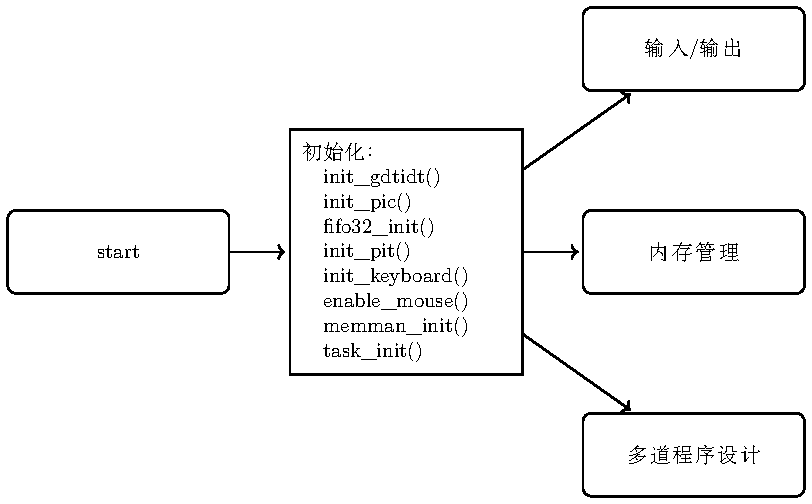
\includegraphics[width=.8\textwidth]{../Fig/func/run.pdf}
  \caption{操作系统组件功能全览}
  \label{fig:run}
\end{figure}

\begin{description}
  \item[初始化] 初始化过程主要涉及到:\\
  内存的损坏检测,数据情况,系统数据写入;\\
  输入设备中键盘及鼠标的启用等;
  \item[内存管理] 包括内存的分配和释放;
  \item[输入输出] 包括对键盘和鼠标输入的处理,以及标准输出;
  \item[多道程序] 包括多道程序设计,分时系统,程序切换及程序的优先级设置。
\end{description}

% 内核
\chapter{编写操作系统内核}

从内存管理,输入输出,多进程,分时四个模块丰富操作系统的内容

\section{内存管理}

内存 (RAM) 是计算机中不可或缺的重要硬件,所有程序的运行都是在内存中进行的,
而CPU访问硬盘数据也必须先经过内存交换才得以实现,内存在加速CPU访问硬盘居功至伟。
由内存的重要性可知内存管理在操作系统中也非常重要。	

内存管理设计的主要目的是快速并且高效的分配内存空间,并在适当的时间释放并回收内存空间。
根据内存管理的设计目的,内存管理的数据结构如下:

\begin{listing}[H]
  \inputminted[tabsize=2, firstline=137, lastline=143,
  linenos=true]{c}{../ZOS/src/kernel/bootpack.h}
\end{listing}

\begin{description}
\item[frees:]可用信息数目
\item[maxfrees:]用于观察可用状况:frees的最大值
\item[lostsize:]释放失败的内存的大小总和
\item[losts:]释放失败次数
\end{description}

经过内存初始化和释放所有内存空间后,内存管理正常运行。

\subsection{内存分配}


\begin{listing}[H]
  \inputminted[tabsize=2, firstline=68, lastline=80,
  linenos=true]{c}{../ZOS/src/kernel/memory.c}
\end{listing}

\subsection{内存释放}

为保证磁盘空闲空间尽可能不呈现碎片化,内存释放主要分为三种情况:

\begin{description}
\item[前端空闲:]释放内存的相连前端是空闲内存或释放内存相连两端都是空闲内存
\item[后端可用:]释放内存的相连后端是空闲空间
\item[前端后端均不可用:]挪动空闲空间以合并
\end{description}

已知:待释放的空间的开始地址和空间大小

遍历内存,直到
当待释放的空间free[i]前方
\newpage

前端空闲如图\ref{fig:mem0}和图\ref{fig:mem1}所示: 

\begin{figure}[h]
  \centering
  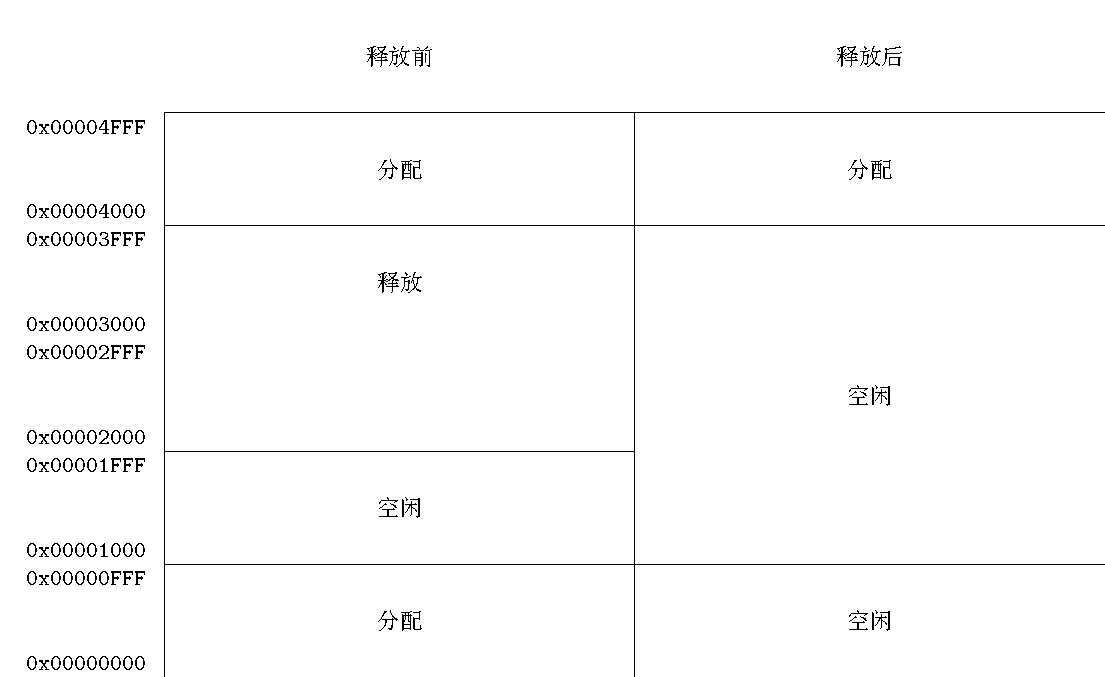
\includegraphics[width=.7\textwidth]{fig/mem0.pdf}
  \caption{前端空闲}
  \label{fig:mem0}
\end{figure}

\begin{figure}[h]
  \centering
  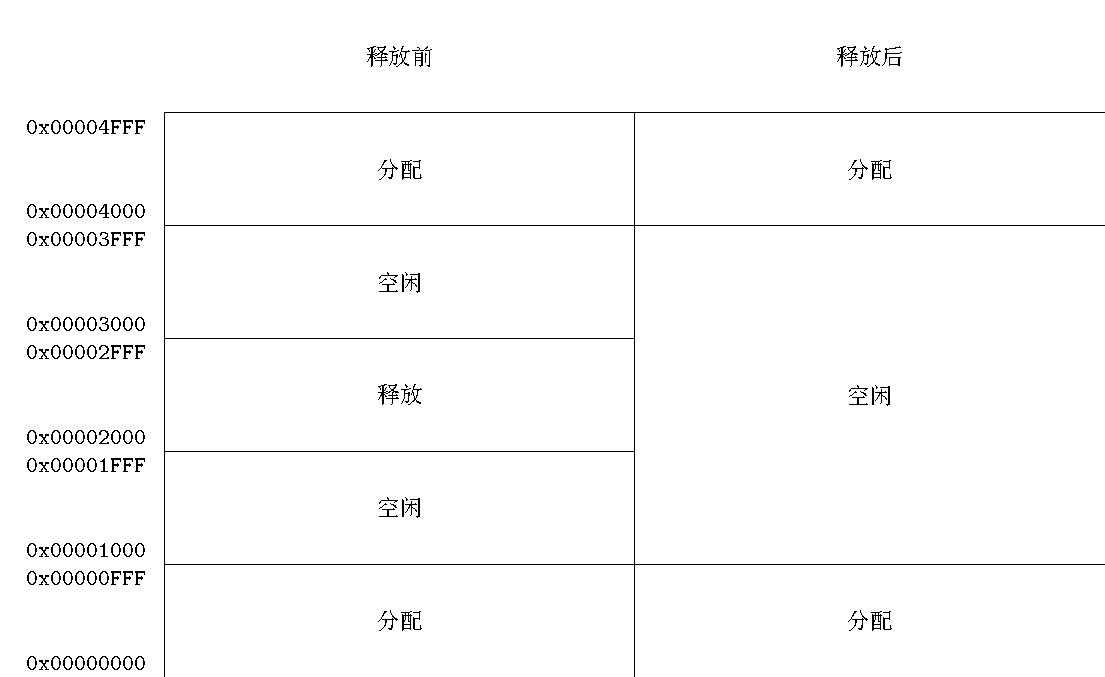
\includegraphics[width=.7\textwidth]{fig/mem1.pdf}
  \caption{前端可用,且后端空闲}
  \label{fig:mem1}
\end{figure}

实现如下:

\begin{listing}[H]
  \inputminted[tabsize=2, firstline=98, lastline=116,
  linenos=true]{c}{../ZOS/src/kernel/memory.c}
\end{listing}

后端空闲:

\begin{figure}[h]
  \centering
  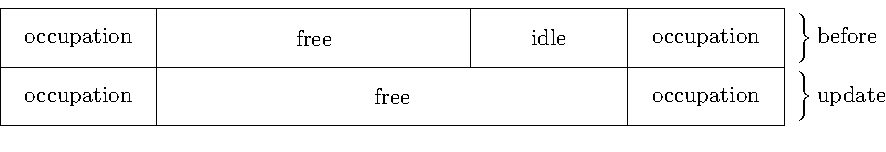
\includegraphics[width=.7\textwidth]{fig/mem2.pdf}
  \caption{后端空闲}
  \label{fig:mem3}
\end{figure}

实现如下:

\begin{listing}[H]
  \inputminted[tabsize=2, firstline=118, lastline=127,
  linenos=true]{c}{../ZOS/src/kernel/memory.c}
\end{listing}

前端后端均被占用:

\begin{figure}[h]
  \centering
  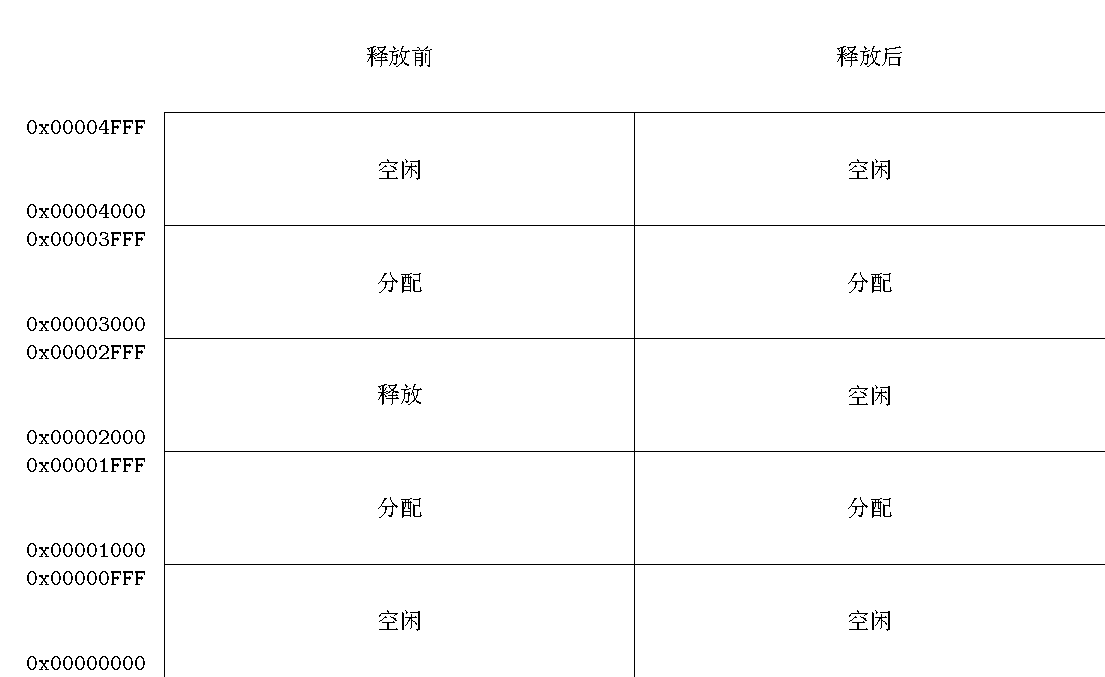
\includegraphics[width=.7\textwidth]{fig/mem3.pdf}
  \caption{前端后端均被占用}
  \label{fig:mem4}
\end{figure}

实现如下:

\begin{listing}[H]
  \inputminted[tabsize=2, firstline=128, lastline=141,
  linenos=true]{c}{../ZOS/src/kernel/memory.c}
\end{listing}

\section{输入输出}

输入作为人与计算机之间最基本的交互方式,其中键盘和鼠标作为标准输入设备。

\subsection{键盘输入}

\begin{listing}[H]
  \inputminted[tabsize=2, firstline=162, lastline=170,
  linenos=true]{c}{../ZOS/src/kernel/bootpack.c}
\end{listing}

\subsection{鼠标输入}

\begin{listing}[H]
  \inputminted[tabsize=2, firstline=247, lastline=265,
  linenos=true]{c}{../ZOS/src/kernel/bootpack.c}
  \inputminted[tabsize=2, firstline=329, lastline=338,
  linenos=true]{c}{../ZOS/src/kernel/bootpack.c}
\end{listing}

\subsection{标准输出}


\section{多道程序系统}

现代的计算机已经不仅仅作为数字计算的工具,而进入大众生活的计算机被赋予了更多的生活需求,
用户可能在看电影的同时查看电子邮件,也有可能在写论文的时候进入浏览器查询相关资料,
但是更重要的是计算机往往在用户不经意间打开防病毒软件等保证用户计算机的安全\cite{tanenbaum2009modern}。

由此可见多进程的工作方式在计算机工作中同样不可或缺。

但是在实际的处理过程中,计算机并不能同时处理多个程序,所以必须采用分时的设计,
关于分时操作系统的设计在下一节。
在此有两个概念,同时处理和多个程序,同时处理属于分时,多道程序属于多道程序设计。

首先要处理的问题是如何在运行多个程序,。

\section{分时操作系统}

在上一节中说到分时是使得在用户看来计算机的多道程序同时运行,多道程序已经实现了,
分时简单说是使得CPU在用户不能明显感觉到的时间间隔内切换运行多个程序,在切换的过程中...


% 兼容
\chapter{实现对外兼容及安全防护}

从接口设计及安全防护的角度完善操作系统
    

%%% 正文部分到此结束。下面是『参考文献』、『指导教师简介』、『鸣谢』、『附录』

%% 不要动下面四行!
\Appendix{}
\printbibliography[heading={bibintoc},title={参考文献}] % 输出参考文献
\advisorinfopage{}                 % 输出指导教师简介
\acknowledgmentspage{}             % 输出鸣谢

%%% 下面是附录部分,可以没有。

% 附录
\chapter{文件清单}

\section{根目录}
\begin{description}
    \item[includes/] 调用的C函数库
    \item[kernel/] 系统kernel目录
    \item[apps/] 系统调用演示程序
    \item[demos/] 系统测试程序
\end{description}

\section{Kernel目录}
\begin{description}
    \item[asmhead.nas]                                                                                                                                        
    \item[bootpack.c] 主程序                                                                                                                                      
    \item[bootpack.h] 头文件                                                                                                                                           
    \item[dsctbl.c] GDT,IDT控制程序                                                                                                                                          
    \item[fifo.c] 缓冲区                                                                                                                           
    \item[file.c] 文件管理                                                                                                                                            
    \item[graphic.c] 图像显示及控制                                                                                                                                     
    \item[int.c] 中断                                                                                                                                             
    \item[ipl09.nas] 启动程序IPL                                                                                                                                         
    \item[keyboard.c] 键盘控制                                                                                                                                       
    \item[memory.c] 内存管理                                                                                                                                          
    \item[mouse.c] 鼠标控制                                                                                                                                           
    \item[mtask.c] 多程序控制                                                                                                                                           
    \item[naskfunc.nas] 汇编函数库                                                                                                                                      
    \item[sheet.c] 图层控制                                                                                                                                           
    \item[timer.c] 定时器                                                                                                                                           
    \item[window.c] 窗口控制
\end{description}







% 程序
\chapter{主要程序代码} %附录二

\section{初始启动程序代码(ipl09.nas)节选}
\label{sec:ipl09.nas}
\begin{listing}[H]
  \inputminted[tabsize=2, firstline=12, lastline=29,
  linenos=true]{nasm}{../ZOS/src/kernel/ipl09.nas}
  \caption{FAT12格式磁盘专用代码}
  \label{sec:fat12}
\end{listing}

\begin{listing}[H]
  \inputminted[tabsize=2, firstline=76, lastline=88,
  linenos=true]{nasm}{../ZOS/src/kernel/ipl09.nas}
  \caption{将磁盘内容读入内存}
  \label{sec:read}
\end{listing}

\begin{listing}[H]
  \inputminted[tabsize=2, firstline=138, lastline=147,
  linenos=true]{nasm}{../ZOS/src/kernel/ipl09.nas}
  \caption{读取磁盘数据到内存}
  \label{sec:readfrag}
\end{listing}

\section{内存管理程序代码(memory.c)节选}

\begin{listing}[H]
  \inputminted[tabsize=2, firstline=68, lastline=78,
  linenos=true]{c}{../ZOS/src/kernel/memory.c}
  \caption{分配内存}
  \label{lst:alloc}
\end{listing}

\begin{listing}[H]
  \inputminted[tabsize=2, firstline=91, lastline=95,
  linenos=true]{c}{../ZOS/src/kernel/memory.c}
  \caption{确定采取何种方式释放内存}
  \label{lst:rw}
\end{listing}

\begin{listing}[H]
  \inputminted[tabsize=2, firstline=98, lastline=116,
  linenos=true]{c}{../ZOS/src/kernel/memory.c}
  \caption{前端可用}
  \label{lst:mem1}
\end{listing}

\begin{listing}[H]
  \inputminted[tabsize=2, firstline=118, lastline=127,
  linenos=true]{c}{../ZOS/src/kernel/memory.c}
  \caption{后端空闲}
  \label{lst:mem2}
\end{listing}

\begin{listing}[H]
  \inputminted[tabsize=2, firstline=128, lastline=141,
  linenos=true]{c}{../ZOS/src/kernel/memory.c}
  \caption{前端后端均被占用}
  \label{lst:mem3}
\end{listing}

\end{document} % 结束。不要动下面几行!

%%% Local Variables:
%%% mode: latex
%%% TeX-master: t
%%% End:
